% !Mode:: "TeX:UTF-8"   %%winedt 以utf8编码打开
% Can only be compiled with xelatex+bibtex

%双行标题
\documentclass[twoside,longtitle]{LZUthesis}
%单行标题
%\documentclass[twoside]{LZUthesis}

\usepackage{float}
\usepackage{fancybox}
\usepackage{calc}
\usepackage{mathdots}
\usepackage{graphicx}
\usepackage{listings}

%声明图片后缀名
\DeclareGraphicsExtensions{.pdf,.eps}

\makeatletter

% 设置图形文件的搜索路径
\graphicspath{{figures/}}

% 小节标题靠左对齐
\CTEXsetup[format+={\flushleft}]{section}

% 取消链接的颜色(黑白打印时启用)
%\hypersetup{colorlinks=false}

%使文档居中,打印时应注释掉
\evensidemargin 0.93 true cm
\setlength{\hoffset}{-0.3 cm}

%允许equationarray分页换行
\allowdisplaybreaks

%使字体清晰,且透明位图不会使页面文字粗细不一
\usepackage{eso-pic}
\AddToShipoutPicture{%
\special{pdf: put @thispage <</Group << /S /Transparency /I true /CS /DeviceRGB>> >>}%
}

%页面背景色
%\definecolor{yellow}{rgb}{0.99,0.99,0.70}
%\pagecolor{yellow}

%浮动项超链接正确跳转
\usepackage[all]{hypcap}

\makeatother


\begin{document}

%分类号;一般不要求学生填写
\classification{}

%密级;申请保密后需填写
\confidential{}

%中文标题
\title{兰州大学研究生学位论文}

%中文标题第二行,题目较短时删除之,并去除文档类选项 longtitle
\titleadd{\LaTeX{}模板简介}

%英文标题
\englishtitle{Introduction to the \LaTeX{} Template of}

%英文题目第二行,题目较短时删除之,并去除文档类选项 longtitle
\englishtitleadd{Lanzhou University Thesis}

%作者汉语姓名
\author{XXX}

%专业
\major{物理学•理论物理}

%学位
\degree{博士}

%研究方向
\direction{XXXX}

%导师姓名+职称
\advisor{某某某~教授}

%论文工作起止年月
\datebeginAndEnd{2012年9月至2015年5月}

%论文提交日期
\submitdate{}

%答辩日期
\defenddate{}

%学位授予日期
\degreedate{}

%左侧页眉
\lzuthesis{兰州大学博士学位论文}

%生成封面
\maketitle

%生成声明页
\makestatement

%前文-罗马页码
\frontmatter\pagenumbering{Roman}

%中文摘要
\begin{abstract}
本文是兰州大学学位论文的\LaTeX{} (包含LyX)模板及其使用说明。除了介绍文档类LZUthesis的用法外,本文还是一份简要的学位论文写作指南。
\end{abstract}

%中文关键词
\keywords{兰州大学,学位论文,\LaTeX{}模板,LyX模板}

%英文摘要
\begin{englishabstract}
This paper is a \LaTeX{} (include LyX) thesis template of Lanzhou University. Besides the usage of the LaTeX document class LZUthesis, a brief guideline for writing the thesis is also included.
\end{englishabstract}

%英文关键词
\englishkeywords{Lanzhou University, Thesis, \LaTeX{} Template, LyX Template}

%自动生成章节目录以及pdf书签
\tableofcontents{}


%正文部分-数字页码
\mainmatter

%正文页眉页脚样式
\pagestyle{lzu}


\chapter{引言\label{chap:intro}}

虽然兰州大学研究生院制定了\href{http://ge.lzu.edu.cn/degree/xwsq/lwgf/201103/1186.htm}{学位论文撰写要求},但只提供了\href{http://ge.lzu.edu.cn/degree/xwsq/lwgf/201103/1187.htm}{~Word 模板}。广大理科生更加青睐的\LaTeX{}却没有标准模板。\href{http://blog.sciencenet.cn/home.php?mod=space&uid=117412&do=blog&id=512804}{LZUthesis~} 宏包是赵振华以中科院学位论文宏包\href{http://www.ctex.org/PackageCASthesis}{~CASthesis~}作为基础模板,根据兰州大学研究生院学位论文撰写要求修改的。作者对LZUthesis宏包进行了进一步修改(主要变更见附录~\ref{chap:changelog}~及\href{https://github.com/mosesnow/LZUthesis/commits/master}{~Github~}),使之更加符合兰大学位论文的撰写要求,并制作了相应的LyX模板。

宏包底层使用的是Xe\LaTeX{},而不是CJK方案,原因在于:
\begin{enumerate}
\item Xe\LaTeX{}支持系统字体,对中文友好。
\item Xe\LaTeX{}支持unicode,可编译各国文字。
\item Xe\LaTeX{}支持常见的图片格式,如:pdf、eps、jpg、png 等。
\end{enumerate}


模板使用LyX的优点是所见即所得,比较直观,缺点是\TeX{}中一些复杂功能难以实现。另外LyX可以导出标准的\TeX{}代码(参见第~\ref{sec:export}~节),方便转入\TeX{}编辑器继续撰写。

青睐\TeX{}模板的用户,直接编辑模板根目录下的Thesis.tex即可。注意它不是Thesis.lyx直接导出的,如果要使用此模板,不要让LyX导出\TeX{}时覆盖此文件。


\chapter{系统配置}

\texttt{LZUthesis}宏包使用了宏包amsmath、amsthm、amsfonts、amssymb、bm、ctex 和hyperref。目前大多数的\TeX{}系统中都包含有这些宏包。但是中文字体在各个系统中却不尽相同:Windows 下使用C\TeX{} 套装一般不需要额外配置字体,但Linux 和Mac一般情况下需要设定中文字体,中文字体名称可通过命令~\lstinline!sudo fc-list :lang=zh-cn!~ 查看,具体配置见本章内容。请注意字体设定可能要根据你自己系统的中文字体做相应调整。


\section{Windows配置}
\begin{itemize}
\item 安装C\TeX{}套装,最新的版本可以从\href{http://www.ctex.org}{~www.ctex.org} 网站下载。
\item 安装完成后,把所有宏包升级到最新(开始菜单--CTEX--Update(Admin))。
\item 安装LyX,最新的LyX安装包可以从\href{http://www.lyx.org/Download}{~www.lyx.org/Download} 下载。
\end{itemize}

\section{Linux配置}

软件安装以ubuntu为例,其他发行版应根据具体情况安装。
\begin{itemize}
\item 安装texlive以及texlive-lang-cjk。


\doublebox{\begin{minipage}[t]{0.86\textwidth}%
\begin{lstlisting}[language=bash,breaklines=true]
sudo apt-get install texlive texlive-xetex
sudo apt-get install texlive-lang-cjk
\end{lstlisting}
%
\end{minipage}}

\item 安装LyX。


\doublebox{\begin{minipage}[t]{0.86\textwidth}%
\begin{lstlisting}[language=bash,breaklines=true]
sudo apt-get install lyx
\end{lstlisting}
%
\end{minipage}}

\item 中文字体设置

\begin{enumerate}
\item 文档类选项(文档--首选项--文档类)中添加选项{[}nofonts{]}
\item 导言区(文档--首选项--\LaTeX{}导言区)中添加(Forked from\href{https://bitbucket.org/kevinyounglzu/latextemplateoflzuthesis}{~Kevin Young's tempalte})


\tiny
\begin{center}
\hrule


\begin{verbatim}


\setCJKmainfont[BoldFont=文泉驿微米黑,ItalicFont=文泉驿正黑] {文泉驿正黑} \setCJKsansfont{文泉驿微米黑}
\setCJKmonofont{文泉驿等宽正黑}
\setCJKfamilyfont{zhsong}{文泉驿正黑}
\setCJKfamilyfont{zhhei}{文泉驿微米黑}
\setCJKfamilyfont{zhfs}{文泉驿等宽微米黑}
\setCJKfamilyfont{zhkai}{文泉驿等宽正黑}
\newcommand*{\songti}{\CJKfamily{zhsong}} % 宋体
\newcommand*{\heiti}{\CJKfamily{zhhei}}   % 黑体
\newcommand*{\kaishu}{\CJKfamily{zhkai}}  % 楷书
\newcommand*{\fangsong}{\CJKfamily{zhfs}} % 仿宋


\end{verbatim}


\hrule
\end{center}
\normalsize

\end{enumerate}
\end{itemize}

\section{Mac配置}
\begin{itemize}
\item 安装Mac\TeX{},最新安装文件可以从\href{https://tug.org/mactex/}{~https://tug.org/mactex/}
网站下载。
\item 安装LyX,最新的LyX安装包可以从\href{http://www.lyx.org/Download}{~www.lyx.org/Download} 下载。
\item 中文字体设置

\begin{enumerate}
\item 文档类选项(文档--首选项--文档类)中添加选项{[}nofonts{]}
\item 导言区(文档--首选项--\LaTeX{}导言区)中添加(Forked from\href{https://bitbucket.org/kevinyounglzu/latextemplateoflzuthesis}{~Kevin Young's tempalte})


\tiny
\begin{center}
\hrule


\begin{verbatim}


\setCJKmainfont[BoldFont=Heiti SC Light,ItalicFont=Kaiti SC]   {Songti SC Light}
\setCJKsansfont{Heiti SC Light} \setCJKmonofont{Songti SC Light}
\setCJKfamilyfont{zhsong}{Songti SC Light}
\setCJKfamilyfont{zhhei}{Heiti SC Light}
\setCJKfamilyfont{zhfs}{STFangsong}
\setCJKfamilyfont{zhkai}{Kaiti SC}
\newcommand*{\songti}{\CJKfamily{zhsong}} % 宋体
\newcommand*{\heiti}{\CJKfamily{zhhei}}   % 黑体
\newcommand*{\kaishu}{\CJKfamily{zhkai}}  % 楷书
\newcommand*{\fangsong}{\CJKfamily{zhfs}} % 仿宋


\end{verbatim}


\hrule
\end{center}
\normalsize

\end{enumerate}
\end{itemize}




\chapter{模版使用}


\section{模板文件结构\label{sec:files}}

整个模板根目录的文件列表如下:

\begin{tabular}{|l|l|l|l|}
\hline
LZUthesis.cls & ---LZUthesis宏包 & \textcolor{red}{{*}} & \textcolor{magenta}{\$}\tabularnewline
\hline
LZUthesis.cfg & ---LZUthesis宏包配置文件 & \textcolor{red}{{*}} & \textcolor{magenta}{\$}\\
\hline
LZUthesis.layout & ---LZUthesis的LyX布局文件 & \textcolor{red}{{*}} & \textcolor{magenta}{\$}\\
\hline
CASmthesis.cls & ---CASthesis宏包 & \textcolor{red}{{*}} & \textcolor{magenta}{\$}\\
\hline
CASmthesis.cfg & ---CASthesis宏包配置文件 & \textcolor{red}{{*}} & \textcolor{magenta}{\$}\\
\hline
lzubib.bst & ---引文样式文件 & \textcolor{red}{{*}} & \textcolor{magenta}{\$}\\
\hline
bib/thesis.bib & ---bib数据库 & \textcolor{red}{{*}} & \textcolor{magenta}{\$}\\
\hline
figures/lzu.pdf & ---兰州大学校名标准字 & \textcolor{red}{{*}} & \textcolor{magenta}{\$}\\
\hline
Thesis.lyx & ---LyX模板主文件 & \textcolor{red}{{*}} & -\\
\hline
Envelope.lyx & ---A3封面LyX模板 & \textcolor{red}{{*}} & -\\
\hline
spine.lyx & ---书脊LyX模板 & \textcolor{red}{{*}} & -\\
\hline
Thesis.tex & ---\TeX{}模板主文件 & - & \textcolor{magenta}{\$}\\
\hline
Makefile & ---Makefile文件 & - & -\\
\hline
gbt7714-2005.bst & ---符合国标gbt7714-2005的引文样式文件 & - & -\\
\hline
\end{tabular}

注:\textcolor{red}{{*}}表示LyX模板必须的文件,\textcolor{magenta}{\$} 表示\LaTeX{}模板必须的文件。


\section{基本设置}
\begin{enumerate}
\item 模版默认使用的文档类选项(文档--首选项--文档类--自定义)是twoside,~longtitle,即双面,长标题。

\begin{enumerate}
\item 双面:此时页码、页边距以及章开始页等会对奇偶页区别设置,可更改为oneside。
\item 长标题:若标题较短时应去除选项longtitle,并删除中英文标题的第二行。
\end{enumerate}
\item 图片搜索路径默认设置为模板根目录下的figures/。
\item bib数据库默认设置为模板根目录下的bib/thesis.bib。
\end{enumerate}

\section{示例}

论文中最常使用的一些功能在本节中给出示例,其他LyX功能的使用详见帮助-- 用户手册,\TeX{}使用则可参考The \TeX{}book\cite{Knut04-T}。


\subsection{公式}

自旋玻色模型的哈密顿量为
\begin{equation}
\hat{H}=\frac{\epsilon}{2}\hat{\sigma}_{z}-\frac{\Delta}{2}\hat{\sigma}_{x}+\sum_{k}\omega_{k}\hat{b}_{k}^{\dagger}\hat{b}_{k}+\sum_{k}\frac{g_{k}}{2}\hat{\sigma}_{z}(\hat{b}_{k}+\hat{b}_{k}^{\dagger})\label{eq:sbm}
\end{equation}



\subsection{表格}

前五个希腊字母
\begin{table}[H]
\begin{centering}
\begin{tabular}{|c|c|c|c|c|}
\hline
Alpha & Beta & Gamma & Delta & Theta\\
\hline
$\alpha$ & $\beta$ & $\gamma$ & $\delta$ & $\theta$\\
\hline
$A$ & $B$ & $\Gamma$ & $\Delta$ & $\Theta$\\
\hline
\end{tabular}
\par\end{centering}

\protect\caption{希腊字母表\label{tab:Greek}}


\end{table}



\subsection{图形}
兰州大学校名标准字
\begin{figure}[H]
\begin{centering}

\includegraphics[width=0.618\textwidth]{figures/lzu}
\par\end{centering}

\protect\caption{兰州大学校名标准字\label{fig:lzu}}
\end{figure}



\subsection{引用}


\subsubsection{交叉引用}

对所有需要引用的公式、表格、图形,执行插入--标签后,即可使用插入-- 交叉引用自动产生引用。
\begin{itemize}
\item 哈密顿量见方程~(\ref{eq:sbm})。
\item 希腊字母表见表~\ref{tab:Greek}。
\item 校名标准字如图~\ref{fig:lzu}。
\end{itemize}

\subsubsection{文献引用}

将引文的bib数据库(默认文件名为thesis.bib)放入模板根目录下的bib 文件夹,即可通过插入--文献引用自动产生引文。
\begin{itemize}
\item Journal:An article\cite{Liu13PRA-A}。
\item Book:C\TeX{} FAQ\cite{Wu05-C}。
\end{itemize}

\subsection{Makefile}

Makefile(Forked from\href{https://bitbucket.org/kevinyounglzu/latextemplateoflzuthesis}{~Kevin Young's tempalte})仅限\LaTeX{}模板编译使用,适合Linux和Mac用户使用。
\begin{enumerate}
\item make:只编译源文件,快速调试用。
\item make ref:包含引用的完整编译。
\item make clean:清除临时文件。
\end{enumerate}

\section{注意事项}
\begin{enumerate}
\item 模板目录下的必须文件(见第~\ref{sec:files}~节)注意不要删除。
\item 请尽量升级\TeX{}宏包到最新,一些旧包会使排版稍微不正常。截止到\today ,此模板在最新宏包下工作正常。
\item Bibkey中不能有中文字符。
\item LyX中必须用空格时,尽量用\textasciitilde{}或(插入--格式-- 强制间距~) 代替,不用空格的原因是:LyX不会中文断句,使用空格将使得LyX编辑界面混乱。
\item Hyperref已经在模板中声明过,如果在LyX中执行插入--超链接会造成冲突(直接编辑\TeX{}代码无此问题),这时只能通过插入\TeX{} 代码的方式使用,比如:\lstinline!\href{https://www.google.com}{Google}!。
\item LyX中,enumerate环境结束后,必须先添加一个分割线环境才能换行,具体参见第\ref{chap:intro}章中列表结束后的蓝色分割线(蓝色分割线仅现于LyX)。
\end{enumerate}

\section{论文打印}


\subsection{文档设置}
\begin{enumerate}
\item 按需选取twoside或者oneside的选项。
\item 文档类notypeinfo选项去除typeinfo。
\item 启用导言区(文档--首选项--\LaTeX{}导言区)的~\lstinline!\hypersetup{colorlinks=false}!以取消链接的颜色。
\item 预留左侧装订线:注释掉导言区中如下两行


\doublebox{\begin{minipage}[t]{0.86\textwidth}%
\begin{lstlisting}[language=bash,breaklines=true]
\evensidemargin 0.93 true cm
\setlength{\hoffset}{-0.3 cm}
\end{lstlisting}
%
\end{minipage}}

\end{enumerate}

\subsection{书脊生成}
\begin{enumerate}
\item spine.lyx生成竖排的书脊文字。
\item Envelope.lyx生成含书脊的封皮,纸张大小A3+。
\item 若中文标题中含有英文,需要将导言区(文档--首选项--\LaTeX{} 导言区)中的\lstinline!\shuji! 替换为如下样式:\footnotesize
\begin{lstlisting}
\shuji[某\hspace{0.3em}\raisebox{-5pt}{English}\hspace{-0.1em}~某]
\end{lstlisting}
\normalsize 本文标题中的\LaTeX{}即是如此处理,对于全中文标题的情况可做上面的相反替换。
\end{enumerate}


\chapter{技术分析、机器学习与中国市场的弱有效}
Fama(1970)\cite{Malkiel1970EFFICIENT} 中提及了一种判断金融市场是否具备有效性的方法,那就是通过判断技术分析所形成的交易策略盈利能力,来判断市场是否达到了弱有效。该文献总结了之前的研究者对道琼斯工业指数施加算法交易所产生的效果。其中,有一种交易策略称之为“百分比滤波”($y\%$ filter)。这个简单的交易算法是一个追涨杀跌的模型,它的操作方法如下所描述:当操作的标的物上涨了$y\%$,则选择追高买入。等到股票从最高点回撤$y\%$时,就选择卖出,不论盈亏。这里的$y$是一个可变动的参数,合理的$y$似乎可以构造一个可盈利的系统,但Fama认为,这样一套交易算法难以从市场中盈利。\\
本文将从机器学习的视角来重新解构技术分析的内涵,并提出一个全新的基于机器学习和人工智能(artificial intelligence)的技术分析交易模型。本章将逐步介绍这样一种交易算法,以及最终判定该交易算法是否有效的,这涉及到了时间序列随机化因果推断的方法。同时,以往对于市场有效性的研究多将目光聚焦于股票指数,但股票指数即便是有效的,也不能代表单独购买特定的普通股没有投资机会。因此,本文将考察1600余例股票走势数据,并采用多种基于机器学习的数据挖掘方法,以全面探讨技术分析的盈利性。
\section{用机器学习来理解技术分析}
Fama的这个研究中,有一个细节:$y\%$ filter中的$y$的大小是可变的,文中使用栅格点搜索(grid search)的方法考察了$y$从0到50的、以0.1为间隔的所有取值。这在一定程度上精确地还原了技术分析的真实的特点。但近期的研究者却放弃了对参数进行栅格点搜索,而仅仅是用少数几种参数组合来代表一整套的技术分析方法,进而再对技术分析的盈利能力进行判断。

文献\cite{sunbibo2004}通过分析三种技术分析策略的盈利能力来判断中国股票市场的有效性,对有限的参数组合、有限的标的物来进行了考察,但最终仍然找到了统计意义上显著的盈利方式。文献\cite{linlijia2019}则对移动平均线交叉的策略在中国A股市场的盈利能力进行了研究,通过对有限的参数组合和不多的标的物时间序列予以研究,认为双均线策略难以在A股市场盈利。以上具有代表性的研究,在他们所研究的某些标的物和技术分析参数下是可以说明问题的,但难以涵盖宏大的技术分析体系,以及丰富的中国股市的多样性。

文献\cite{chenfangfang2019}将MACD,RSI,OBV等传统的技术分析学派常用的技术指标作为特征,引入到了支持向量机(SVM)模型之中,产生了较好的预测效果。文献\cite{Patel2015Predicting}则比较了SVM、人工神经网络(ANN)、随机森林(random  forest)以及朴素贝叶斯(naive-Bayes)等模型对股票指数进行预测的效果,并得出了随机森林的效果为最佳的结论,与文献\cite{chenfangfang2019}一致,该研究也使用了传统技术分析指标来进行特征工程(feature engineering)。上述文献将传统技术分析所产生的指标与机器学习领域中的各类方法相结合,取得了不错的预测效果。

但不论是直接使用简单的技术分析交易系统作为对A股市场的有效性进行判断的依据,或者,利用技术分析所带来的技术指标来进行数据编码、降维、特征工程,都忽视了技术分析交易系统本身的弹性和自我进化的生命力。如同机器学习中的可训练权重(weights)和超参数(hyper parameters),技术分析交易系统中各个指标的参数是可变的,甚至可能是随着市场变化而动态调整的。本文将从机器学习领域中,优化的角度来对技术分析进行解读,力图更贴近真实的市场。随后再构建参数可优化的技术分析交易系统。

\subsection{真实市场中的技术分析}
从机器学习的角度来理解,技术分析简单来说分为两个部分,第一部分是依据市场数据进行数据挖掘,以得到决策系统所需要使用的材料;第二部分,则是依据之前挖掘得到的材料,构建具体的策略系统。当然,真实世界中的复杂交易系统要更为复杂。可以将技术分析产生交易决策与围棋游戏中,AI根据盘面形势进行判断并最终产生决策进行类比。因此,技术分析决策产生的过程也可以类比Deepmind机构在2017年发表的文献\cite{Silver2017Mastering}中所描述的AI决策产生的过程。
\[
i_{t-1} &= f_{\theta}(s_{t-1}, s_{t-2}, ...),\\
a_t &= \pi (i_{t-1}).
\]\\
其中,$s_t$表示t时刻的市场数据汇总,经典技术分析框架下,$s_t$常常包含t时刻的开盘价(open)、收盘价(close)、最高价(high)、最低价(low)以及成交量(volume),这些数据可用于画蜡烛图,进而通过道琼斯波浪或艾略特波浪理论以及各类技术分析形态来捕捉特征信号,也可用于计算指标。$f_\theta$则是将市场信息进行加工,提取信号(signal)或指标值,这些特征可以被作为交易决策的依据。

$\pi$则是一个策略系统,输入$i$得到交易决策$a$。值得注意的是,$t$时刻的交易决策只能依据$t-1$及之前的信息来产生。量化交易领域,对策略进行回测(backtest)时,应当注意未来函数,未来函数是需要坚决避免的,使用未来函数进行回测,无法准确判断策略的有效性。未来函数最常见的例子就是收盘价(close),和各大行情软件中显示出来的移动平均线。因为收盘价应当在蜡烛图的一个bar走完后才最终确定,回测如果使用了当前bar的收盘价,则使用了未来数据。

从机器学习的角度,信号提取的过程$f_\theta$的骨架常常是确定了的,而可学习的地方就是参数$\theta$,但技术分析系统中,这些参数常常是不可导的,甚至,我们还需要另外定义一个损失函数(loss function)。因为,技术分析本质上不是简单地预测,而是需要产生交易行为以获得盈利,因此,本文定义负盈利(negative profit)作为技术分析交易系统的损失函数。
\[
l(\theta)=\mathbf{NP}=-\mathbf{Pf}\left(a_{t}(\theta), p_{t}, p_{t+1}, ..., p_{t+d}\right).
\]
上式中,$\mathbf{NP}$就是负利润,而$\mathbf{Pf}$则是利润。技术分析在真实市场中的表现形态复杂多样,真实市场中,优秀的$f$、$\theta$以及优秀的资金管理策略和交易算法都是盈利的关键所在。可以将真实市场中的技术交易系统的步骤进行如下总结,本文将根据以下简化了的技术分析交易系统构建策略:
\begin{itemize}
	\item 由技术分析系统盯市,并产生交易信号
	\item 产生信号后,对信号进行过滤或二次确认
	\item 接入买入算法交易模块
	\item 接入卖出策略、风险控制等模块
\end{itemize}
产生这样一个技术分析交易系统,往往是经过市场数据回测检验和实盘检验,并进行参数调整后,确认了可以赚钱才会上线。因此,技术分析系统的参数具有动态性。本文将把$\theta$视为可学习的,而学习目前就是上式中的损失函数最小化。

\subsection{技术分析与特征提取及选择}
特征提取(feature extraction)源自传统的计算机视觉领域。在深度学习(deep learning)兴盛之前,基于传统机器学习以及特征提取、特征工程技术的机器视觉曾经是计算机视觉领域占据统治地位的方法。机器学习专家常常会以特征工程的方式,捕捉图形的特征以供下一步计算。这些特征的类型有:边缘、角、区域等等。机器学习专家还设计对应的算法,对特征进行特征选择(feature selection),之后再运用支持向量机(support vector machine)或逻辑回归(logistic regression)等分类算法或回归算法,最终完成对图形进行分类或回归的任务。

技术分析则是精明的投资者对于股价长期变化进行观察积累的理论化了的经验,从机器学习的角度来进行分析,技术分析无外乎对金融市场中的历史交易数据进行数据挖掘。而此数据挖掘的第一步是特征提取,这与计算机视觉中的人工特征工程有异曲同工之妙。
\begin{table}[H]
	\centering
	\caption{常见技术指标}
\begin{tabular}{|c|c|}
	\hline
	类型 & 技术指标 \\
	\hline
	大势型 & ABI、ADL、ADR、MSI、STIX等 \\
	\hline
	超买超卖型 &  CCI、乖离率、相对强弱指标、W\&R等\\
	\hline
	趋势型 & DMA、DMI、TRIX、VHF、VPT等 \\
	\hline
	能量型 &  VCI、OBV、VR、MAD等\\
	\hline
	成交量型 &  成本分布、ADVOL、PVT、SSL等\\
	\hline
	均线 &  EXPMA、MA、VMA、LMA等\\
	\hline
	图表型 &  K线、等量K线、宝塔线、红三兵、三只乌鸦等\\
	\hline
\end{tabular}
\end{table}
todo excel to latex;

对股票价格的OLHC数据进行特征提取有很多方法,常见的特征有:均线(MA)、相对强弱指标(RSI)、随机指标(KDJ)等。技术分析指标琳琅满目,本文使用的技术分析指标为移动平均线,其的计算方法为:
\begin{equation}
	\mathbf{MA}_k &= \frac{1}{k}\sum_{i=1}^{k}C_{t-i}
\end{equation}
下图是一个双移动平均线的示例,图中使用的是平安银行(股票代码:000001.SZ)的数据,使用windquant notebook画出。其中,深色的实线是5日均线,而浅色的实线是35日均线。一个简单的均线交易系统所产生的信号可能是:当5日均线上穿35日均线时,产生买入信号;当5日均线下破30日均线时,产生卖出信号。

值得一提的是,技术分析领域所谈的上穿,其实还有一个隐含条件,那就是均线呈多头向上趋势。也就是,均线值需要满足以下条件:
\begin{equation}
\mathbf{MA}_{k,t} \le \mathbf{MA}_{k,t-1}\\
\mathbf{MA}_{l,t} \le \mathbf{MA}_{l, t-1}
\end{equation}
todo 换行;式号;
多头排列这个条件在很多有关均线的研究中被忽视了。

\begin{figure}
	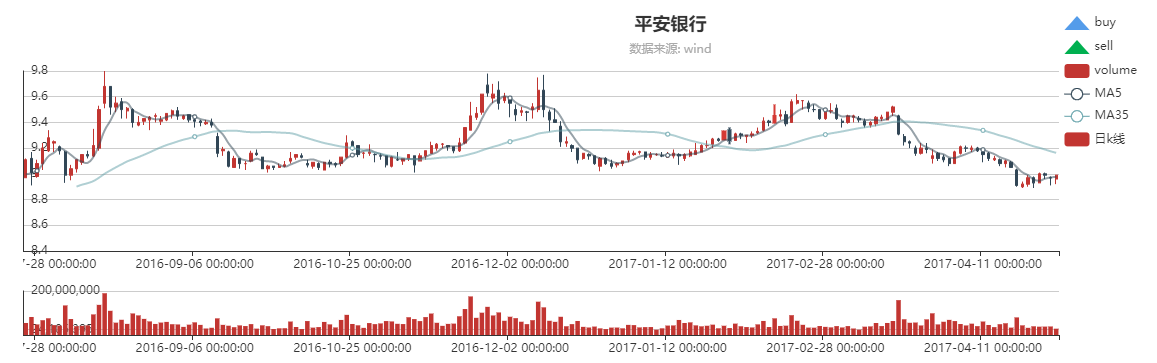
\includegraphics[scale=0.5]{figures/ma_exp.png}
	\caption[移动平均线示例]{移动平均线示例}
	\label{fig:maexp}
\end{figure}

从上文可以看出,技术分析指标种类繁多,不同类型的指标可能适用于不同的标的物(例如:指数、蓝筹股、小盘股)。老练的技术分析者完全可能通过对不同股价走势的同时观察,由此产生多个技术指标信号成为交易决策的依据,从而实现对多个股票的市场数据挖掘。

除了以上琳琅满目的技术指标外,技术分析专家还可以通过观察蜡烛图的形态和颜色,找到一些形态类的特征。例如:M头、W底、圆弧底、头肩底、红三兵、三只乌鸦、仙人指路等等。形态类利用的数据实质上是OLHC蜡烛图数据。形态类的特征还有波浪理论,波浪理论通过对之前行情的“波浪”进行计数,以判断当前牛市(或熊市)的绝对位置。均线或平滑异同移动平均线(MACD)等的技术指标也可绘制成副指标图,形成了多头排列、空头排列、金叉、死叉等被技术分析派认为反映了市场多空力量对比的特征。

技术分析者研究得出的技术分析特征具有一定价值,陈等在2019年引入了MACD、RSI等传统技术分析形成的特征\cite{chenfangfang2019},再使用随机森林(random forest)和boosting等方法执行了预测任务,最终获得了较好的效果。需要注意,仅是特征提取并不能完整地囊括技术分析的所有流程。

提取了特征后,老练的技术分析交易者会根据自己的经验和见闻来对特征进行取舍。以上所列的一系列技术分析特征,最终只被保留很少的部分,作为技术分析者使用的交易系统的基石。需要注意,简单的交易系统往往是特定市场环境下,经过技术分析玩家长期的市场实践,优胜劣汰留下的系统,其涵义与研究者随机抽取的交易系统存在区别。因为,长期市场的优胜劣汰实则为交易系统的演进提供了温床。

\section{技术分析与参数优化}
市场人士普遍认为,技术分析如果可以盈利,那么盈利的关键要素一定不是指标或系统,而是运用技术分析的老练的交易者。例如,有一种基于技术分析的交易方法被称之为炒单。炒单的意思是,交易者完全凭借自己脑海中复杂的神经网络系统,根据市场上盘口数据的信号,直接依赖直觉捕捉交易机会,以博取差价。技术高超的炒单员可能积少成多、聚沙成塔,达到稳定盈利的目标。\\
\begin{figure}
	\centering
	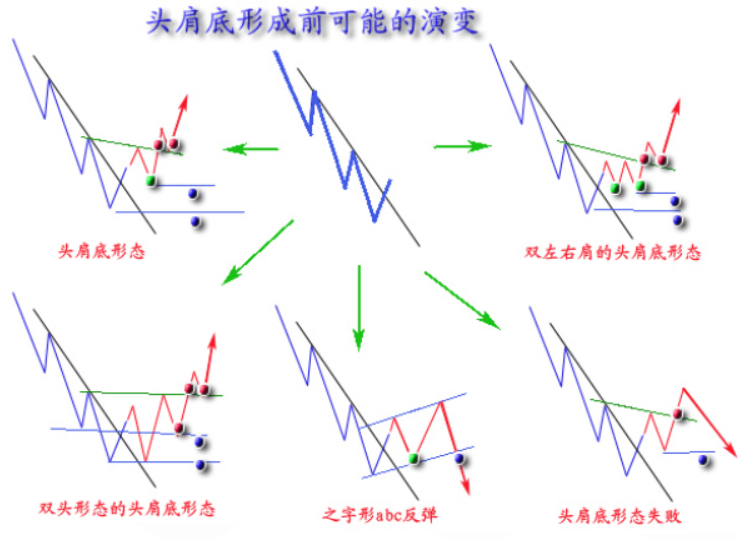
\includegraphics[width=0.7\linewidth]{figures/ta-1.png}
	\caption{金融标的价格走势的底部形态\footnote{图片来源于新浪博客 http://blog.sina.com.cn/u/6013942202}}
	\label{fig:ta-1}
\end{figure}
基于价格走势图形的直觉式下单,或称炒单,则是市场数据挖掘的一种极端的形式。这个极端的形式对于$s_{t-1}$的挖掘直接通过人脑的极端复杂的超大规模的神经网络来进行。这个超大规模的生物神经网络的权重和参数是由交易员累积的经验所习得的,与本文在机器学习的视角下,对技术分析体系进行参数优化的方法颇有类似。

对于直觉式下单,或称“炒单”,目前没有足够的研究材料。但对于高频交易的下单问题,人工交易也是大型量化投资机构的选项。

Bojinov等在2017年分析了某大型量化投资机构的人工交易与算法交易的优劣,该文章构造了随机化的时间序列实验方法以及因果估计目标(causal estimand),据此对比了人工交易与算法交易的金融滑点(slippage)的优劣\cite{Iavor2019Time}。该研究的结果是,某些任务中,人工交易滑点更低,而某些任务则相反。

从市场的角度来理解,人工下单的执行力和反应速度都是不及算法的,但人类的直觉式下单可以在复杂环境下对当前局面进行直觉性的判断,也具备迅速举一反三的小样本学习能力,这是算法难以做到的。因此,在算法交易所考验的低市场冲击、隐藏交易信息等方向,人类的直觉也并非一无是处。

从机器学习的角度来看,技术分析的指标或形态,仅仅能提供一个分析框架,机器学习模型最终的预测效果,有赖于数据驱动(data-driven)产生的训练后的权重。

在机器学习的框架下,如果我们有$N$个训练样本:$\{(x_1,y_1),...,(x_N,y_N)\}$。这里,$x_i$是第$i$个样本的训练样本,而$ y_i $则是第$ i $个目标(target)。机器学习此时需要寻找一个函数$ g(x) $,使得$ g(x)=\arg\min_y \mathcal{L}(x,y) $。其中,$ \mathcal{L} $是损失函数,一般是函数$g$的拟合优度。

\begin{equation}
R_{emp}(g)=\frac{1}{N}\sum_i \mathcal{L} (y_i, g(x_i))
\end{equation}

如何定义损失函数$\mathcal{L}$,以及,如何寻找$g$,就是机器学习所关心的问题。对于这个问题,最常见的解决方法是经验风险最小化(empirical risk minimization)或称为损失函数最小化(loss minimization)\cite{Vapnik2000The}。上式就是经验风险的表达式。经验风险最小化通常会使得函数$g$最优地切合训练数据。但如果函数$g$过于注重切合训练数据,往往就会造成对于新数据的预测能力的下降。这在机器学习领域被称为过拟合(overfitting)。对此,统计学家采用结构化的风险最小化(structure risk minimization)来寻找$g$,具体来说,结构化风险在确定$\mathcal{L}$上做文章,常常会引入惩罚项(panalty)来控制预测方差,提升模型的泛化能力,或称模型上线后的表现。有关泛化能力的定义如下式:
\begin{equation}
R_{online}(g)=\frac{1}{M}\sum_i \mathcal{L}(y_i, g(x_i)),
\end{equation}
其中,$M$是新数据的个数。最终,机器学习的学习目标是产生具有优秀泛化能力的模型,泛化能力好的机器学习模型具有以下两个特点:
\begin{itemize}
	\item $ R_{emp}(g) $足够小;
	\item $R_{online}(g)$与$ R_{emp}(g) $的差距足够小;
\end{itemize}

在目力所及的范围内,本研究属于首次将机器学习与技术分析进行类比的研究。因此,本文的模型并不复杂,因此,暂时不引入惩罚项(penalty)或其他对抗过拟合的手段。本文所构建的基于技术分析交易系统的优化模型,基于以上机器学习中,监督学习(supervised learning)的基本算法,以下就是基本的算法。
\begin{enumerate}
	\item 确定$ s_i, f, \pi $
	\item 确定$\mathcal{L}(\theta)$为负利润
	\item 寻找$\theta$以将$\mathcal{L}$最小化
\end{enumerate}
这里,$ s_i $是第$i$时刻所包含的有关的市场信息,可以是市场信息(价格系信息、成交量系信息),也可以包括市场公告等场内信息,甚至也可能包含场外的信息。理论上说,全世界在$i$时刻以前所产生的信息都可以包含在内。但在实际运用这个算法的过程中,由于金融市场数据本身的特点,我会使用$i-1$时刻的市场信息作为特征输入,以防止运用到了未来函数。

$f$此处是指技术分析的交易系统,例如:双均线系统。每个系统都会带有可变的参数,之前已提及,一个朴素的双均线策略应当包含对$ma_1$和$ma_2$周期的动态调整。

$\theta$是可变的参数,这与机器学习领域的表示方法不太一样。在机器学习领域中,$\theta$常常用来表示超级参数或翻译为超越参数(hyper parameter),这些超级参数一旦确定,在训练过程中则是不可变的,但,选择合理的超级参数又是机器学习领域进行落地实践时的一个亟需解决的大问题。本文对于技术分析参数的搜索方法也借鉴自机器学习中的超级参数选择的相关算法。

$\pi$是指策略生成函数,策略生成函数根据技术分析框架对市场信息产生的信号来生成交易策略,这包含了买卖策略和下单策略。本文在不影响结论的前提下,不考虑边角情况(corner case),假设所有证券和资金都是可无限分割的。本文所使用的买卖策略和下单策略就是简单的全仓进出,在不考虑边角情况的条件下,以上策略的回测是十分方便的。

$\mathcal{L}$是指损失函数,此处是指负利润。该损失函数不存在封闭的计算方法,而需要经过策略回测(backtest)得到。策略回测是指将$\pi$所生成的策略用于新的历史数据(未用于训练的数据)的模拟交易,并引入合理的滑点和交易成本设置,最终产生盈亏。由此算出来的负利润就是本文所定义的损失函数。

\section{参数优化的实现}
在机器学习领域,系数或权重(weights)(类比于本文技术分析体系中的参数)的优化方式有多种。经典线性模型中,满足一定条件下,权重的最优解存在闭式解(close-formed)。对于岭回归而言,我们也可以通过矩阵运算,高效地求出解析解。岭回归是防止线性回归出现过拟合,降低泛化误差的一种有效手段,它实际上是引入了inductive bias来帮助算法更为正确的理解实际情况。

对于以下损失函数的优化:
\begin{equation}
||Ax-b||_2^2 + ||\Gamma x||_2^2
\end{equation}
其中,$x$是可变的系数,Tikhonov矩阵$\Gamma$是经过合理选择的。此Tikhonov回归存在显式解,写作$\hat{x}$,

\begin{equation}
\hat{x}=(A^{T}A+\Gamma^{T}\Gamma)^{-1}A^{T}b.
\end{equation}

但是,复杂的机器学习算法中,让损失函数最小化的权重往往是不存在显式解(explicit solution)的。甚至,损失函数本身可能也不是凸(convex)的,或者是不光滑(smooth)的,这意味着可能存在多个局部最优解。对于反向传播神经网络(BP neural network),常见的优化方法是基于反向传播的梯度下降(gradient descent)算法。

梯度下降算法有很多变体,机器学习领域,基于一阶梯度的算法有:随机梯度下降(Stochastic Gradient Descent)、动量(momentum)、Nesterov加速算法、Adam、AdaGradient等等。这些算法中,Adam是实际效果最好的\cite{Kingma2014Adam}\cite{Nesterov2017Efficiency}。统计机器学习领域,最小角回归算法(least angle regression)实际上也是一种梯度下降算法\cite{Tibshirani2004Least},实际上,LAR算法是让系数朝着拥有最大梯度的坐标方向移动,而当存在两个梯度一样的方向时,先动某一个方向则意味着下一次会移动另一个方向,如果学习率趋近于0,则最终会形成系数坐标沿着角平分线路径运动的效果。

梯度下降为基础的优化算法(gradient based method)是当今机器学习领域几乎仅存的优化策略,但本文所研究的技术分析交易系统,其损失函数$\mathcal{L}$需要通过回测求得,梯度更是无从谈起。因此,我们需要通过其他的方法对技术分析交易体系的参数进行优化。

而自Fama\cite{Malkiel1970EFFICIENT}从上世纪中叶开展有效市场理论的研究以来,大多数研究对于技术分析的设定和定义都是参数静态的。而对参数的调整也是技术分析交易系统的一部分,甚至,参数的调整和确认可能是比交易系统本身更为重要的一部分。不调整参数的技术分析交易模型,就像是未经精调(fine-tuning)的深度学习模型,其效果不能代表技术分析的真正实力。

前文提到,人类的直觉在交易领域依旧占据一席之地。同理,也可以通过模拟人类直觉调参的方式来对技术分析交易系统进行优化。如同围棋游戏,人类通过棋感和围棋知识来缩小搜索范围,技术分析参数的确定,也可以理解为和alphago\cite{Silver2017Mastering}类似的缩小状态空间(state space)的搜索范围的问题。因此,本文将顺着这个思路,一步一步解决机器学习的参数优化问题。

下面,我先来构建一个朴素的双均线交叉策略:
\begin{enumerate}
	\item 定义 $MA_{k,t}=(1/m_k)\sum_{i=t-m_k-1}{t-1}p_i $,其中,$k=1,2,3,4$;
	\item 定义 $y_1\%, y_2\%$;
	\item 买入信号:$MA_{1,t-1}>MA_{2,t-1}$;
	\item 买入信号确认:$MA_1$和$MA_2$呈上升趋势,其$t-1$时刻的一阶差分大于等于0;
	\item 过滤信号:$MA_{3,t-1}>MA_{4,t-1}$
	\item 产生买入信号后,如果信号得到了确认,且经过了过滤,则全仓买入。
	\item 退出策略:当股价上升$y_1\%$后,盈利退出;当股价下降$y_2\%$后,止损退出。
\end{enumerate}

对以上交易算法,我们需要调整6个参数,分别是$m_1,m_2,m_3,m_4,y_1,y_2$。使得定义的经验损失$mathcal{L}$最小化。
\begin{equation}
\theta^*=\arg\min_{\theta\in\Theta}\mathcal{L}(p_{new}, \theta),
\end{equation}
其中,$\theta=(m_1,m_2,m_3,m_4,y_1,y_2)$,而$\Theta$是参数空间,代表所有可能的$\theta$取值。一般来说,技术分析体系下,第一条均线被称为快线,代表短期趋势。第二条均线是慢线,代表中期趋势。而过滤信号中的两条均线中,其中一条往往是代表长期趋势或牛熊状态的超慢线。同时,止盈率$y_1\%$和止损率$y_2\%$也有一定的取值范围,一般短期策略的止盈率和止损率都降低,长期策略的止盈率和止损率较高。具体的$\Theta$取值将在本章下一节详细介绍。

求解上式只能通过数值计算的方法。最显而易见的方法就如解决围棋游戏那样,可以通过穷举法(brute-force method)进行搜索。在机器学习领域,这又被成为栅格点搜索(grid search)。栅格点搜索的具体方法是,对于$\Theta$中的所有取值的可能进行离散化,形成一个个格点。本文中,$\Theta$实则是一个高维的多面体。通过对这个多面体内部的离散化的一个个的格点进行遍历,我们就能找到期待的参数组合。

栅格点搜索需要遍历离散化后所有可能的参数组合的取值,因此,计算开销十分巨大。本文所提出的朴素的技术分析策略下,也难以大规模应用栅格点搜索来进行优化。由于栅格点搜索的开销过大,机器学习任务中常见的参数选择方法还有随机搜索(random search)。随机搜索法假设参数服从某种易于抽样(sampling)的概率分布。最简单的随机搜索可以假设参数服从独立的均匀分布,算法将从这个多维分布中不断抽样,达到终止条件后,选择效果最好的参数组合。

以下是随机搜索的参数优化算法\cite{Hastie2004The}。
\begin{enumerate}
	\item 设定所有参数的联合分布$\Pr(\theta|\beta)$(实际应用中,也可假设参数之间相互独立);
	\item 设定迭代次数N;
	\item 进行N次循环,每次都从联合分布中抽取一个参数组合$\theta$;
	\item 从以上产生的参数组合中,选择能让损失函数$\mathcal{L}$最小化的参数组合;
\end{enumerate}

随机参数搜索的运行速度和效率远远高于栅格化搜索,但由于随机噪声的缘故,其准确性相对较差。机器学习领域的自动参数调整,还有一种称为坐标下降的方法。这种方法类似于前向传播的求导方法(forward propagation)。具体的做法是,通过添加扰动观察损失函数的值的变动规律,进而对影响较大的坐标加速下降,而影响较小的坐标则缓速下降。随机参数搜索、栅格点搜索、坐标下降等优化方法,在机器学习领域,尤其是决策树、随机森林、梯度增强决策树、神经网络等较复杂的机器学习模型中应用广泛。

模拟量子退火(simulated annealing)也是一种随机搜索。该算法产生的第一个解是随机生成的,此后,产生的新解由旧解加上随机扰动而产生。产生新解后,算法会判断新解对于目标函数是否有改进。如果有改进,则接受新解,否则,算法将以可变概率拒绝新解,这个概率随着迭代次数的增加而增加。模拟退火算法具有渐进收敛性,已在理论上被证明以概收敛于全局最优解\cite{Hwang1988Simulated}。

那么,现实生活中,老练的技术分析交易者是如何确定技术分析交易系统的参数的呢?答案很可能是直觉。这就像围棋专业九段的棋感一样,老练的技术分析交易者能以少量的迭代步骤找到一个适用于市场的技术分析系统参数。这个过程类似于贝叶斯优化(bayesian optimization)\cite{Pelikan2005Bayesian}。贝叶斯优化常用于损失评估成本较高时的机器学习的调参任务,例如,大型神经网络调参。大型神经网络的训练需要大量的gpu时,成本十分巨大。此时,贝叶斯优化称为了一个有力的工具。贝叶斯优化是当前机器学习、深度学习、数据挖掘领域中,应用最为广泛的超参数(hyper parameter)优化手段。

对技术分析系统进行回测同样是相当耗费算力的,尤其是对于大量时间序列进行事件驱动(event driven)的模拟交易性质的回测。同时,贝叶斯优化于老练的技术分析交易员的调参手段也颇具类似性,老练的技术分析玩家的调参过程与基于序列模型的优化(Sequential model-based optimization,SMBO)有异曲同工之妙,有关SMBO的内容我将在下一小节详细介绍。


人工智能首次战胜职业棋手的算法alphago\cite{2016Mastering}使用了蒙特卡洛树搜索和深度卷积神经网络。Alphago Fan采用了两个神经网络,一个负责评估策略空间,另一个负责评估。因此,这两个网络又被称为策略网络和价值网络。其中,策略网络$p_\sigma$是基于监督学习的,学习的材料是人类的棋谱。对于任何一个局面(state),该策略网络可以返回作为人类,下一步棋可能落子的位置。alphago算法在此基础上进行计算和推演,再运用价值网络进行判断,最终找到算法所认为的最有利于获胜的招法。


真正市场中的技术分析交易系统的参数选择,往往也依赖于技术分析的老手对盘面数据、回测数据的观察,之后采取的跳跃式的、类似神经网络的预测。SMBO算法中的核心是对不同参数组合产生的损失进行预判$p(y|x)$。同时,制定获得函数(acquisition function)主动获得新的参数组合与损失的对应的数据,以进一步将之前的预判准确化。

此处,预判$p(y|x)$类似于一种直觉,以及alphago通过监督学习所训练得到的棋感。而获得函数$S$则需要平衡探索(exploration)和局部优化(exploitation),是基于直觉的一种策略,类似于经验丰富的操盘手调整参数以试探市场获得更多的信息。贝叶斯优化的流程是,从一个参数的实例出发,通过模型来判断可能的结果优秀的下一个参数实例。随后,进行成本较高的结果判断得出$(x_i,y_i)$,再将其整合进数据集$\mathcal{D}$根据新的信息,修正以往的判断模型。再从当前的参数实例出发,寻找下一个可能结果优秀的参数实例,以此类推。

SMBO算法是贝叶斯优化的基本形式,这个算法的核心是找到一个模型,通常是基于统计机器学习的,使得我们可以根据以往的结果来预判可能的结果优秀的参数。目前,常见的模型可以是高斯过程(Gaussian process)甚至可能是随机森林(random forest)或神经网络(feed-forward neural network)。
而技术分析参数的形成也是如此。经验丰富的技术分析者,一开始会使用市场上流传的默认参数,随着时间的推进,他们会观察市场的情况,以此来训练大脑中的真正的生物神经网络。再运用这个神经网络来寻找下一个可能的结果优秀的参数。本文也将通过贝叶斯优化来还原老练的技术分析者调校、打磨其交易系统的过程,并检验最终的决策系统的盈利性。

\section{基于贝叶斯优化的技术分析交易体系}
本文所测试的技术分析交易体系,其参数将是可变的,其中,优化参数的方法基于栅格点搜索、随机搜索和贝叶斯优化。根据上一节中列举的双均线交易算法,我们需调整6个参数,分别是$m_1,m_2,m_3,m_4,y_1,y_2$。分别代表移动平均线的快线周期、慢线周期、用于确认的移动平均线的快线周期和慢线周期,以及止盈比例和止损比例。本文将验证2195只股票总共含有1523667条时间戳数据。

\subsection{基于高斯过程的贝叶斯优化}
贝叶斯优化\cite{Pelikan2005Bayesian}是栅格点搜索、随机搜索以及人工调参的良好替代,其特点是能够在探索(exploration)和最大化利用(exploitation)之间取得均衡。在机器学习领域,贝叶斯优化(bayesian optimization)可被用来优化各种各样的损失函数的交叉验证值,或称交叉验证损失(cv loss),交叉验证损失被认为是泛化误差的一个比较准确的代理\cite{Arlot2009A}。在机器学习领域,损失函数的选择是多样的,可以是基于负对数似然(negative log-likelihood)、精确性(accuracy)或F1得分。本文将从更广义的角度思考问题,所选择的损失函数$\mathcal{L}$是负的交易回报率。

对此,我们需要对求出下列问题的解:
\begin{equation}
x_{opt}=\arg\max_{x\in\mathcal{X}}\mathcal{L}(x),
\end{equation}
此处,方程$\mathcal{L}:\mathcal{X}\rightarrow\mathbb{R}$是一个运算成本很高的函数,这里指交易回测;$\mathcal{X}\subset \mathbb{R}^d$是一个欧式空间内的有界的矩形(box),结合之前的技术分析交易体系$d=6$。贝叶斯优化在实践中被证明适合对随机的、非凸等复杂情况的函数进行优化,且与经验丰富的技术分析交易员人工调参可以类比。以下是基于序列模型的优化(Sequential model-based optimization,SMBO)的具体过程。


\begin{enumerate}
	\item 输入:$\mathcal{L},\mathcal{X}, S, \mathcal{M}$;
	\item 初始抽样:$\mathcal{D}\longleftarrow \mathbf{INIT SAMPLES}(f,\mathcal{X})$
	\item 以下迭代指标从$|\mathcal{D}|$到总样本数循环;
	\item 训练模型$M, \mathcal{D}$,产生$p(y|x,\mathcal{D})$;
	\item 根据获得函数得到$x_i$的值:$x_i=\arg\max_{x\in\mathcal{X}} S(x, p(y|x, \mathcal{D})$;
	\item 得到新数据(这一步成本较高):$y_i=\mathcal{L}(x_i)$, 并将其整合进$\mathcal{D}$;
	\item 重复4-6直到迭代终止。
\end{enumerate}

以上算法中,$\mathcal{L}$就是之前定义的损失函数——负的回报率。其定义为:
\[
\mathcal{L}=-\sum_{i=1}^{T}\log \sum_j\omega_{i, j} r_{i,j}+1,
\]
其中,$\omega_{i, j}$是第$i$个周期,某种标的物所占仓位,而$r_{i,j}$则是该标的物当日的市值变动。在实际处理的过程中,数据是经过了复权处理和其他一些必要处理的。所有标的物的都是以人民币计价的。

投资领域较为关注年化收益率、年化连续复利率等指标,以上损失函数稍加计算便可转化为这些指标。
\[
\mathbf{CCR}=\exp\left(\frac{(\mathcal{-L}+1)}{T}\cdot 365\right)-1,
\]
这里,CCR指代连续复合回报率(Continuously Compounded Rate of Return)。不过从优化的角度来说,由于本文所研究的2000多只股票的周期都是确定的,因此,在实现的过程中直接采用了$\mathcal{L}$作为损失函数。如果所测试的众标的物周期是不固定的,那么,应当采用负的CCR作为对技术分析交易系统进行优化的损失函数。

SMBO算法中的$\mathcal{X}$是一个$d$维的欧式空间中的矩形,但也可以是其他形状,代表各个参数的取值范围的笛卡尔积。$S$指代的是获得函数(acuisition function),这个函数在贝叶斯优化中负责控制探索(exploration)和最大化利用(exploitation)之间的平衡。获得函数的有多种选择方式,常见的有
\begin{itemize}
    \item 高斯过程上置信界(Gassian Process-Upper Confidence Bound,GP-UCB):
    \[
    x_t=\arg\max_{x\in\mathcal{X}}\alpha_t(x)=\arg\max_{x\in\mathcal{X}}\mu_{t-1}(x)+\beta^{1/2}\sigma_{t-1}(x).
    \]
    该获得函数所求最小值的部分,实质上,基于高斯过程的SMBO算法是对$\{x_i\}$建模后求得的后验分布的均值和后验标准差的加权和。其中,$\mu$项是基于已确定的模型的,因此,代表对已有模型的最大化利用(exploitation);$\sigma$项代表对已有模型可能的不确定性的推断,最大化这一项代表对可能产生最优解区域的探索,因此,这一项代表对未知的探索(exploration)。
    \item 期望提升(expected improvement, EI):
    \begin{align*}
    x_t &= \arg\max_{x\in\mathcal{X}}\mathbb{E}_{f(x)\~\mathcal{N}(\mu_{t-1}(x),\sigma^2_{t-1}(x))}[\max(f(x)-f^{+}_{t-1},0)]\\
    &= \arg \max_{x\in\mathcal{X}}(\mu_{t-1}(x)-f^{+}_{t-1})\Theta(\frac{\mu_{t-1}(x)-f_{t-1}^+}{\sigma_{t-1}(x)})+\sigma_{t-1}(x)\phi(\frac{\mu_{t-1}(x)-f_{t-1}^+}{\sigma_{t-1}(x)}),
        \end{align*}
    此处,$\Theta$和$\phi$分别表示标准一元高斯分布的概率密度函数(pdf)和累计分布函数(cdf)。这个式子只考虑提升的可能,在计算期望的时候,过滤掉了导致降低表现的可能,因之被称为期望提升函数。EI的实用性极强,很多实现贝叶斯的软件包使用了EI作为获得函数。
    \item 基于信息论的获得函数\cite{Hoffman2014Predictive}:
    \[
    x_t =\arg\max_{x\in\mathcal{X}}\mathbb{H}\left[p(x_*|\mathcal{D})\right]-\mathbb{E}_{p(y|\mathcal{D}_n,x)}\left[\mathbb{H}[p(x_*|\mathcal{D}_n\cup\{(x,y)\})]\right],
    \]
    此处H表示信息熵,代表信息量或不确定性。该获得函数能获得最大信息量的新样本$x^*$进行高成本的损失函数计算。但实际运算中,由需要对以上获得函数进行近似计算。
\end{itemize}

以上列举了几种可用的贝叶斯优化的获得函数。除了获得函数的不同外,SMBO算法中的回归模型$\mathcal{M}$的也可有差异。目前开放的一些软件包多使用EI(expected improvement)作为获得函数,而回归模型又有多种,例如,高斯过程(Gaussian process)、树结构的Parzen估计(tree Parzen estimation)和随机森林(random forest)\cite{shahriari2015taking}。

\[
\mathbb{E}(R_p)=w_A \mathbb{E}(R_A)+w_B\mathbb{E}(R_B);
\]
\[
\sigma^2_p=w_A^2\sigma_A^2+w_B^2\sigma_B^2+2w_A w_B \sigma_A\sigma_B \prho_{AB} .
\]



以基于序列模型的优化(SMBO)为基础,贝叶斯优化又可根据不同的回归








使得定义的经验损失$mathcal{L}$最小化。



4.1.4 基于神经网络的贝叶斯优化
[todo1] 贝叶斯优化sota
3.2.1 双均线交易系统
本节将使用简单的技术分析交易系统
[todo] 技术分析双均线交易系统
该系统需要优化7个参数,分别是:
[代码需要优化的7个参数]
对这7个参数进行优化的算法如下:
[算法]
数据介绍
回测简述
行情走势与资金权益
3.2.2 海龟交易系统
[todo]


\section{基于贝叶斯优化的机器学习预测及交易算法}

\section{自动技术分析}
类比自动机器学习(auto machine learning),本文提出自动技术分析(auto technical analysis)概念,缩写为autoTA。自动技术分析除了可以自动选择技术分析的指标体系,还应包含模型堆叠、融合等集成学习功能,进一步增强预测能力和稳定性,也更为贴合真实的市场。自动技术分析需要解决以下三个问题:
首先,要彻底将技术分析自动化,需要让技术分析交易系统在一定框架下自由选择技术分析的交易算法。此问题实际上是一个广义的参数选择问题,
其次,集成学习的问题。
成熟的技术分析交易者往往并不依赖于一套交易系统。战胜了人类围棋职业九段的alphago[silver2016]就使用了两套决策系统,一套是基于神经网络的,另一套则是基于传统蒙特卡洛树搜索的。成熟的技术分析交易者往往会融合很多套交易系统,互相参考,以得出稳妥的结论。
从机器学习的角度进行分析,这种交易系统的融合可理解为模型的堆叠(stacking)。机器学习理论证明,训练多个学习器(learning),把弱的学习器组合起来,通常可以达到更好的预测性能。具体而言,套袋法(bagging)可以在预测偏差不变的情况下,有效降低预测方差。而模型增强(boosting)方法,例如,adaboost或GBDT可理解为将新的学习器用于拟合负梯度,实质是一种梯度下降的方法。集成学习在各类数据竞赛中大放异彩。
简单的堆叠(stacking)所涉及的模型数量较小,效果可能不如套袋法或者boosting,但如果技术分析派所堆叠的模型具备一定的多样性(diversity)和准确性(accuracy),哪怕是简单的堆叠则也可大幅降低整个交易系统预测部分的预测方差。
最后,自动机器学习还应解决资金管理和风险控制的问题。
限于篇幅,本文将不具体讨论以上的问题。

3.2 基于机器学习贝叶斯优化的经典技术分析


\chapter{进阶功能}

\section{}


\section{导出\protect\TeX{}\label{sec:export}}

文件-导出-\LaTeX{}(Xe\TeX{}),可导出为tex文件进行进一步编辑,该tex 文件的编译顺序为: Xe\LaTeX{}--Bib\TeX{}--Xe\LaTeX{}--Xe\LaTeX{}。 注意LyX 默认会自动将图片转换为pdf格式,造成一些图片有两个版本,不处理也不会有影响。若想处理,建议保留pdf版本的,因为Xe\LaTeX{}处理pdf图片时,编译速度快;若选择保留其他格式,应在tex文件正文前声明图片的后缀名,比如:\lstinline!\DeclareGraphicsExtensions{.pdf,.eps}!


\section{导入Bibitem到正文}

如果需要在没有bib文件的情况下也可编译,则首先把导出的tex文件完整编译一次,再将生成的bbl文件内容拷贝到tex正文中替换掉如下两行即可

\doublebox{\begin{minipage}[t]{0.86\textwidth}%
\begin{lstlisting}[language=bash,breaklines=true]
\bibliographystyle{lzubib}
\bibliography{bib/thesis}
\end{lstlisting}
%
\end{minipage}}


\section[修复stemV问题]{修复stemV问题\footnote{此问题已在修复透明位图导致文字粗细不一的问题时同时得到解决。}}

由于中文字体某些参数设置不当,\LaTeX{}生成的pdf在Adobe阅读器下中文字体(特别是宋体与仿宋)会稍显模糊,可通过修改stemV值改善。
\begin{enumerate}
\item 下载并安装\href{https://www.pdflabs.com/tools/pdftk-the-pdf-toolkit/}
{~pdftk free}
\item cmd中切换到pdf所在目录,执行


\doublebox{\begin{minipage}[t]{0.86\textwidth}%
\begin{lstlisting}[language=bash,breaklines=true]
pdftk in.pdf output out.pdf uncompress
\end{lstlisting}
%
\end{minipage}}

\item 用文本编辑器编辑out.pdf,查找并修改simsun与fangsong的stemV 值为50,保存。
\item 执行以下命令,得到final.pdf


\doublebox{\begin{minipage}[t]{0.86\textwidth}%
\begin{lstlisting}[language=bash,breaklines=true]
pdftk out.pdf output final.pdf compress
\end{lstlisting}
%
\end{minipage}}

\end{enumerate}

\section{自动生成成果页}
\begin{enumerate}
\item 此方法仅适用于\LaTeX{}模板。
\item 导言中添加:


\doublebox{\begin{minipage}[t]{0.86\textwidth}%
\begin{lstlisting}[language=bash,breaklines=true]
%%自动生成发表文章目录
\usepackage[resetlabels]{multibib}
%把参考文献加入目录中,但排除目录本身
\usepackage[nottoc]{tocbibind}
\newcites{phd}{在学期间的研究成果}
\end{lstlisting}
%
\end{minipage}}

\item 在参考文献列表后添加


\doublebox{\begin{minipage}[t]{0.86\textwidth}%
\begin{lstlisting}[language=bash,breaklines=true]
%%自动生成发表文章目录
%此处插入所有发表文章的bibkey
\nocitephd{Liu13PRA-A}
%定义引文样式为lzubib
\bibliographystylephd{lzubib}
%发表文章的bib库
\bibliographyphd{bib/thesis}
\end{lstlisting}
%
\end{minipage}}

\item 此种情况使用makefile不能完整编译,但WinEdt可以完整编译。执行顺序为:


Xe\LaTeX{}--Bib\TeX{}--Xe\LaTeX{}--Xe\LaTeX{}。


命令行下手动编译时需要额外执行\lstinline!BibTeX phd.aux!。

\end{enumerate}



%附录部分
\appendix

%自动生成参考文献列表,需要模板根目录下有:bib/thesis.bib
\bibliographystyle{lzubib}
\bibliography{bib/thesis}


%致谢
\begin{thanks}
Ajouter de la vie aux jours lorsqu'on ne peut plus ajouter de jours
à la vie.

\begin{flushright}
---Jean Bernard
\par\end{flushright}
\end{thanks}


\chapter{v1.0主要变更\label{chap:changelog}}
\begin{enumerate}
\item 修复目录中摘要和abstract超链接的错误
\item 修复长标题在摘要部分只显示第一行
\item 修复中英文摘要第一行不缩进
\item 修复页眉上不显示完整标题
\item 页眉改为双线
\item 替换lzu.eps为清晰版本
\item 添加lyx模板
\item 修正行间距
\item 设置Twoside时页码在装订线右侧,oneside时居中
\item 调整封面、声明页布局
\item 修正章标题为三号字
\item 改变图表的编号格式为2-1
\item 修正致谢页的字体及行距
\item 修正一些中文字段,如摘要、Key words、在学期间的研究成果等
\item 修改小节标题为不缩进
\item 添加A3封面,书脊
\item 修改bst样式文件
\item 调小装订线距离为0.6cm
\item 致谢、成果偶数页留白
\item 单独定义makestatement
\item 合并cls文件,longtitle作为类选项进入
\item 更改各处全标题的调用
\item 成果页格式调整为与参考文献相同
\item 摘要重定义为chapter,间距微调
\item chapter标题上下间距微调
\item 去除摘要、Abstract、目录的页眉
\end{enumerate}

\end{document}
